\documentclass[10pt]{beamer}

\usepackage[utf8]{inputenc}
\usepackage[spanish, es-tabla]{babel}

\usetheme{metropolis}
\usepackage{appendixnumberbeamer}

\usepackage{booktabs}
\usepackage[scale=2]{ccicons}

\usepackage{pgfplots}
\usepgfplotslibrary{dateplot}

\usepackage{graphicx}

\usepackage{amsmath}
\usepackage{amsfonts}
\usepackage{amssymb}
\usepackage{amsthm}
\usepackage{esvect}

\usepackage{xspace}
\newcommand{\themename}{\textbf{\textsc{metropolis}}\xspace}

\title{The Whale Optimization Algorithm (WOA)}
\author{Ignacio Aguilera Martos}
\date{22 Junio 2018}
\institute{Metaheurísticas}

\begin{document}

\maketitle

\begin{frame}[fragile]{Contenidos}
  \setbeamertemplate{section in toc}[sections numbered]
  \tableofcontents[hideallsubsections]
\end{frame}

\section{Introducción del problema}

	\begin{frame}[fragile]{Competición CEC2014}
		\vspace{10px}
		\pause
		\metroset{block=fill}
		\begin{block}{WOA}
			\begin{itemize}
				\item Algoritmo bioinspirado en cómo cazan las ballenas jorobadas.
				\item Hecho por Seyedali Mirjalili y Andrew Lewis.
				\item Se ejecuta el algoritmo sobre las 20 primeras funciones de CEC2014.
			\end{itemize}
		\end{block}
		\begin{block}{CEC2014}
			\begin{itemize}
				\item Es una competición reconocida a nivel mundial.
				\item Se intenta resolver un problema de minimizacion con 30 funciones.
				\item En nuestro caso sólo lo hemos hecho con dimensión 10 y 30 aunque en la competición se hacía con dimensiones 10,30,50 y 100.
				\item El ganador de la competición fue L-SHADE.
			\end{itemize}
		\end{block}
	\end{frame}

\section{Descripción del algoritmo inicial}

	\begin{frame}[fragile]{Fases de la caza}
		\vspace{10px}
		\pause
		\metroset{block=fill}
		\begin{block}{Fases de la caza}
			\begin{itemize}
				\item Exploración para encontrar presas.
				\pause
				\item Caza de presas.
			\end{itemize}
		\end{block}
		\pause
		\begin{center}
			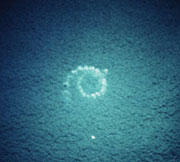
\includegraphics[scale=0.7]{./Imagenes/imagen1.jpg}
			\hspace{10px}
			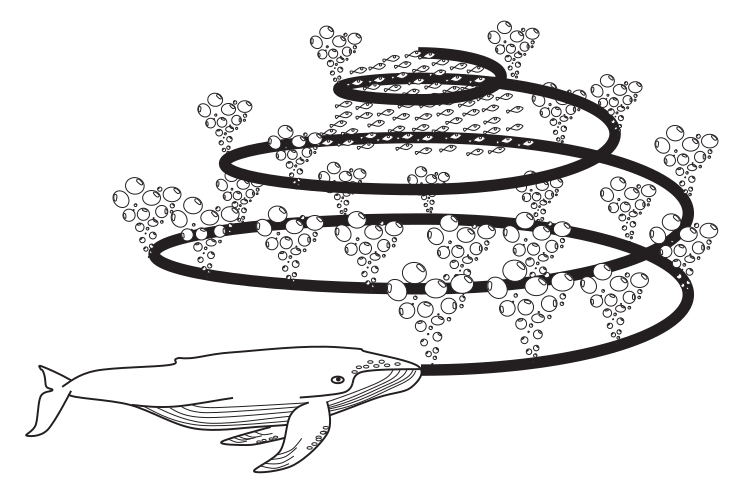
\includegraphics[scale=0.22]{./Imagenes/imagen2.png}
		\end{center}
	\end{frame}

\section{Modelo matemático}

	\begin{frame}[fragile]{Aproximación a la presa}
		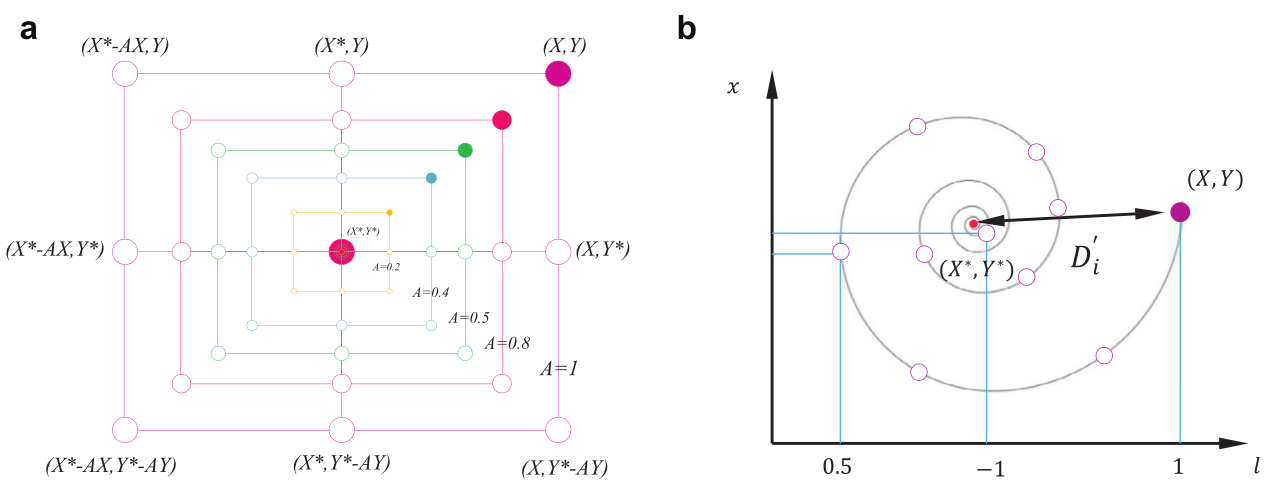
\includegraphics[scale=0.23]{./Imagenes/imagen3.png}
		\pause
		\vspace{5px}
		$D(t) = |\vec{C}\cdot \vec{X^*}(t)-\vec{X}(t)|$ \hspace{20px} $\vec{X}(t+1) = \vec{X^*}(t)-\vec{A}\cdot D(t)$ \\
		\pause
		$D'(t) = |\vec{X^*}(t)-\vec{X}(t)|$ \hspace{20px} $\vec{X}(t+1) = \vec{D'}(t)\cdot e^{bl}\cdot \cos (2\pi l)+\vec{X^*}(t)$ \\
		\vspace{10px}
		$\vec{A} = 2\cdot \vec{a}\cdot \vec{r}-\vec{a}$ \hspace{20px} $\vec{C}=2\cdot \vec{r}$ \\
		\pause
		Donde $X$ es la posición de la ballena, $X^*$ la posición de la presa, $\vec{r}$ un vector aleatorio con valores en el intervalo $[0,1]$ y $a\in [0,2]$ que se decrementa de forma lineal desde 2 hasta 0.
	\end{frame}
	
	\begin{frame}[fragile]{Ecuación real del movimiento}
		\pause
		$$
		\vec{X}(t+1)=
		\begin{cases}
		\vec{X}(t+1) = \vec{X^*}(t)-\vec{A}\cdot D(t) & si \ p<0.5\\
		\vec{X}(t+1) = \vec{D'}(t)\cdot e^{bl}\cdot \cos (2\pi l)+\vec{X^*}(t) & si \ p \geq 0.5
		\end{cases}
		$$
		\pause
		Donde p es un número aleatorio en el intervalo $[0,1]$ \\
		\pause
		En caso de no tener presa hacemos el movimiento lineal hacia una ballena aleatoria.
	\end{frame}
	
	\begin{frame}[fragile]{Pseudocódigo}
		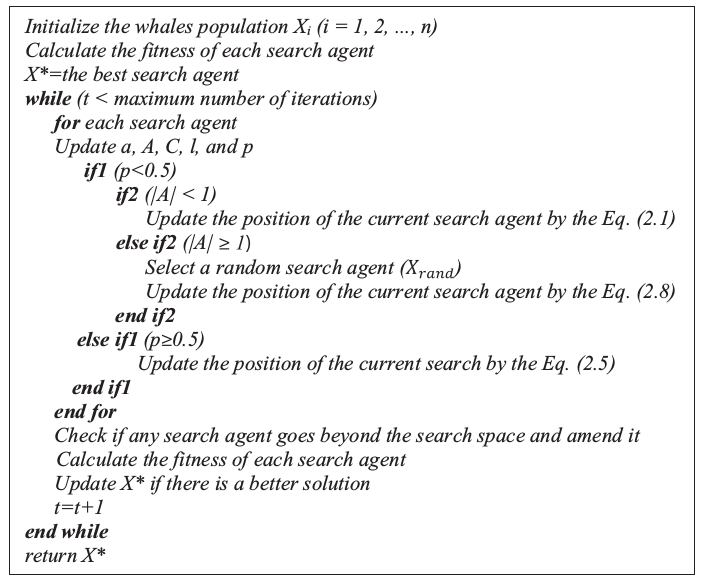
\includegraphics[scale=0.4]{./Imagenes/imagen4.png}
	\end{frame}

\section{Desarrollo de mejoras}

	\begin{frame}[fragile]{Desarrollo de mejoras}
		\vspace{10px}
		\pause
		\metroset{block=fill}
		\begin{block}{Fases}
			\begin{itemize}
				\item Inicialización aleatoria de las ballenas.
				\item Hacer una aproximación espiral a una solución aleatoria al principio del algoritmo.
				\item Incorporación de la búsqueda local Solis Wets.
				\item Incorporación de un esquema de Differential Evolution.
				\item Sustitución de Solis Wets por CMAES.
				\item Reemplazar la aproximación aleatoria para aproximarse a una posición aleatoria del espacio en vez de a una ballena aleatoria.
			\end{itemize}
		\end{block}
	\end{frame}

\section{Versión final}

	\begin{frame}[fragile]{Versión final}
		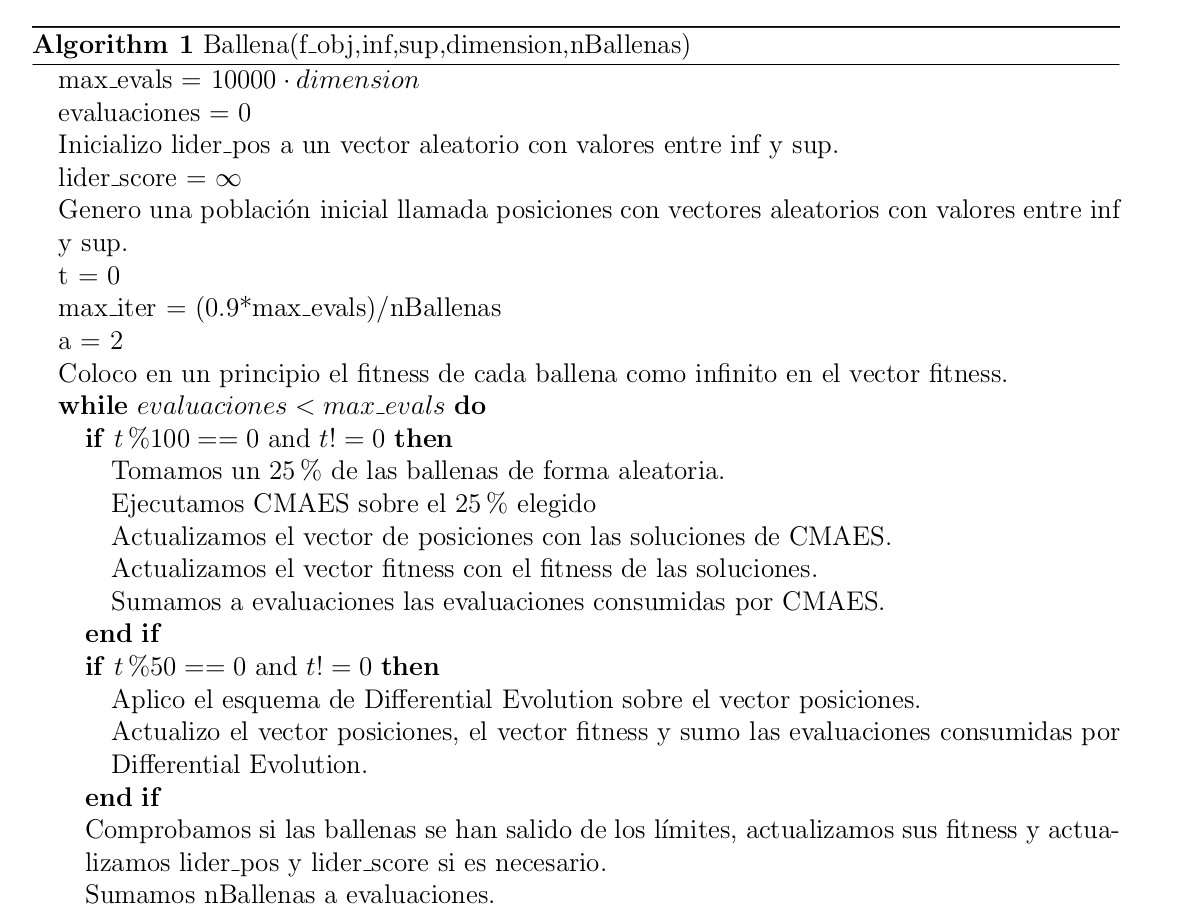
\includegraphics[scale=0.25]{./Imagenes/version_final_p1.png}
	\end{frame}

	\begin{frame}[fragile]{Versión final}
		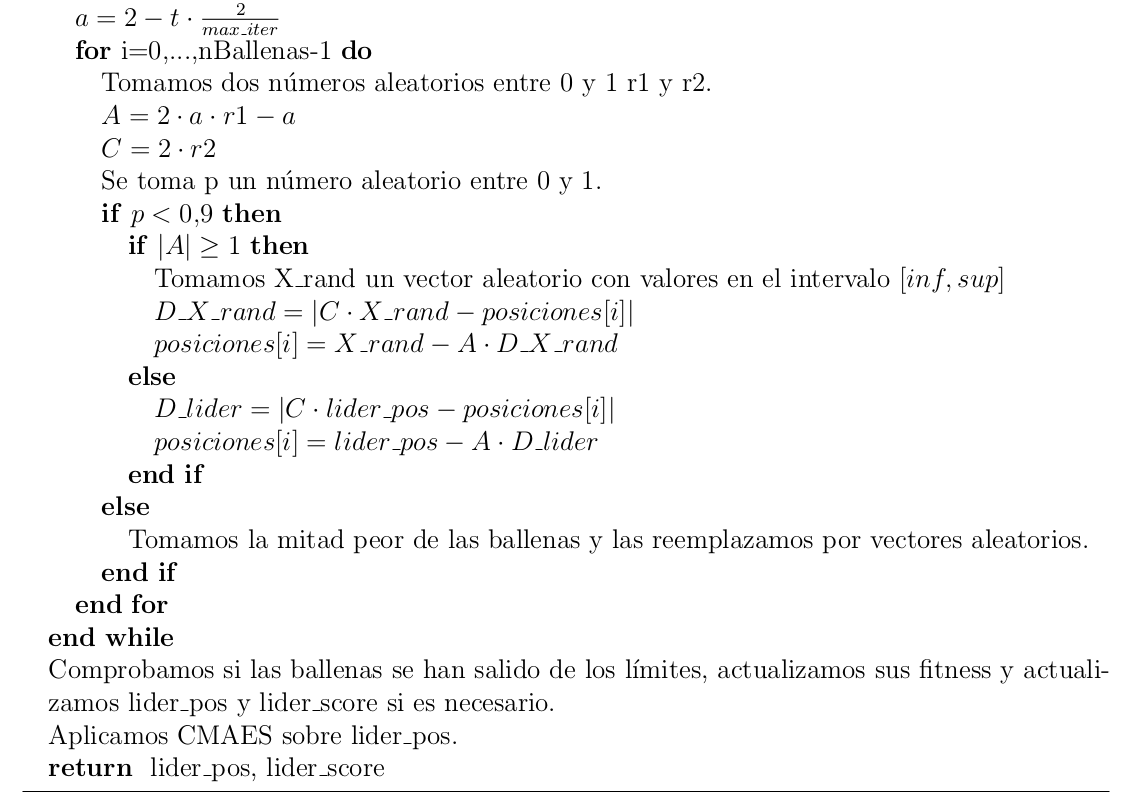
\includegraphics[scale=0.25]{./Imagenes/version_final_p2.png}
	\end{frame}

\section{Resultados}

	\begin{frame}[fragile]{Versión inicial}
		\centering
		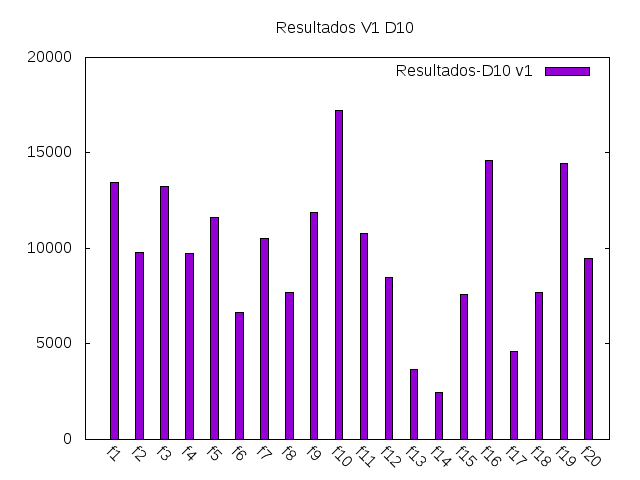
\includegraphics[scale=0.25]{./Imagenes/Resultados/resultados_v1_d10.png}
		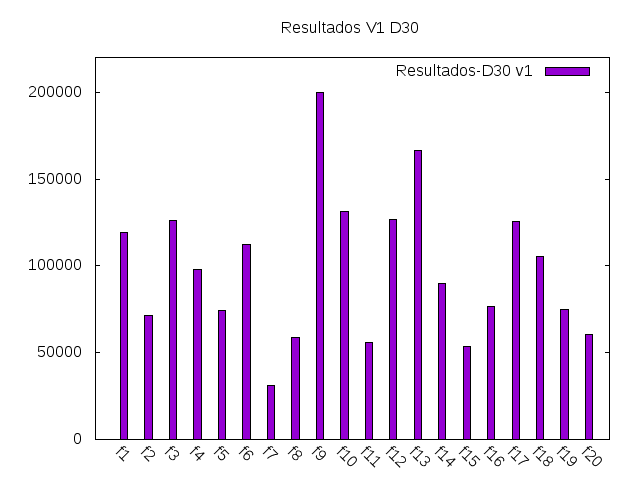
\includegraphics[scale=0.25]{./Imagenes/Resultados/resultados_v1_d30.png}
		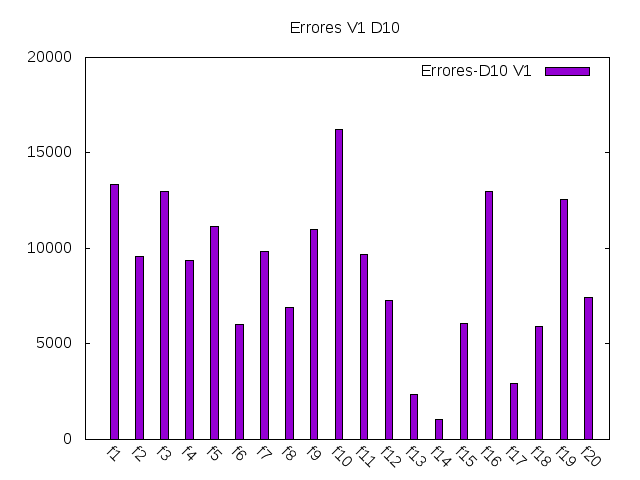
\includegraphics[scale=0.25]{./Imagenes/Errores/errores_v1_d10.png}
		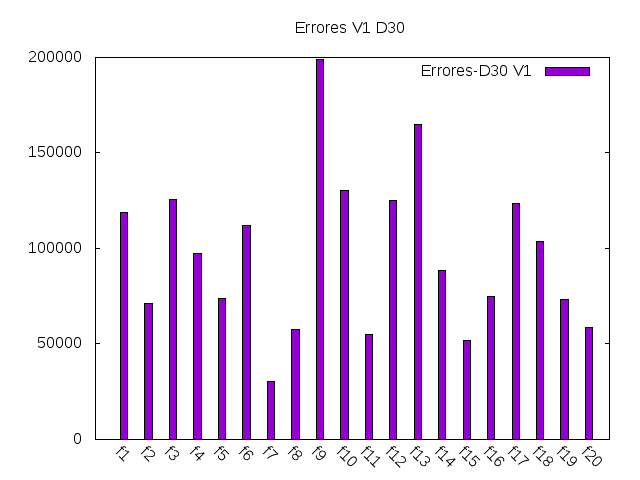
\includegraphics[scale=0.25]{./Imagenes/Errores/errores_v1_d30.png}
	\end{frame}

	\begin{frame}[fragile]{Segunda versión}
		\centering
		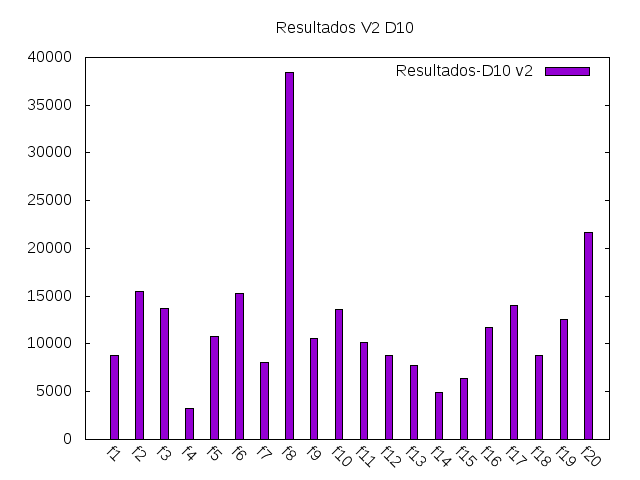
\includegraphics[scale=0.25]{./Imagenes/Resultados/resultados_v2_d10.png}
		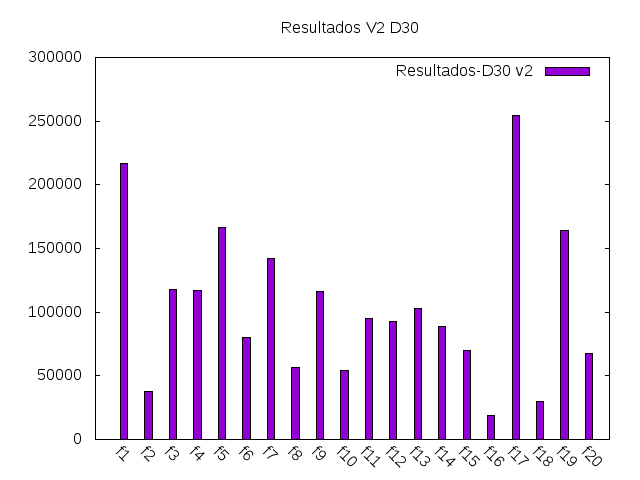
\includegraphics[scale=0.25]{./Imagenes/Resultados/resultados_v2_d30.png}
		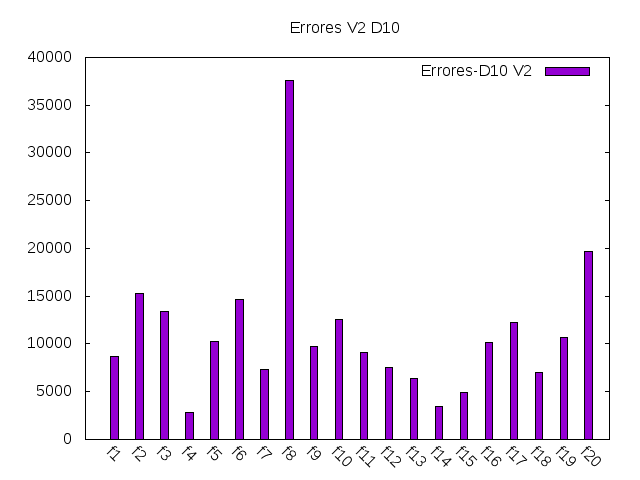
\includegraphics[scale=0.25]{./Imagenes/Errores/errores_v2_d10.png}
		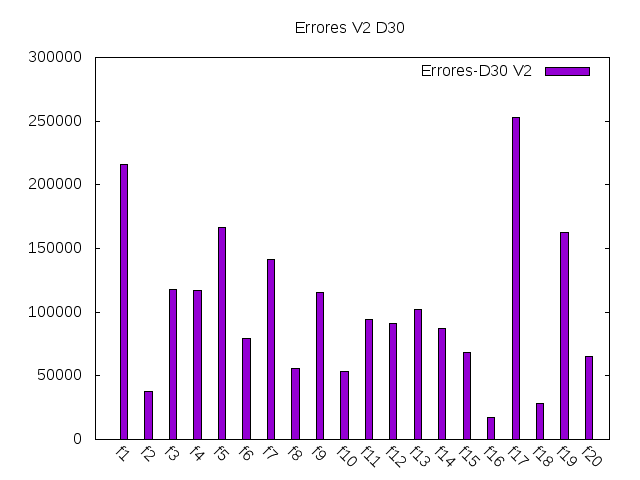
\includegraphics[scale=0.25]{./Imagenes/Errores/errores_v2_d30.png}
		
		\metroset{block=fill}
		\begin{block}{Características}
			\begin{itemize}
				\item Hace una aproximación en espiral a una solución aleatoria.
			\end{itemize}
		\end{block}
	\end{frame}

	\begin{frame}[fragile]{Tercera versión}
		\centering
		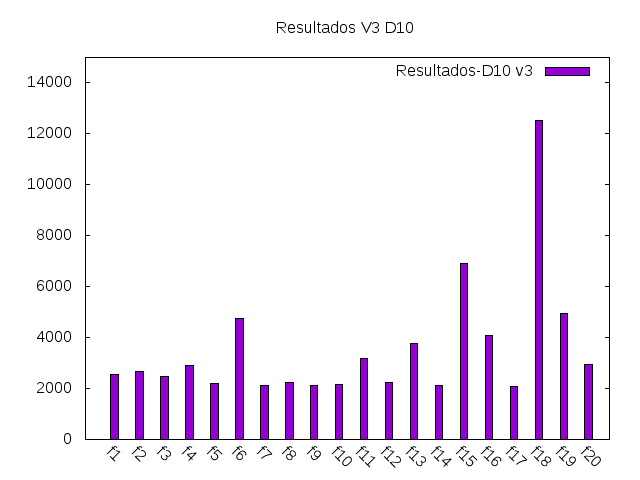
\includegraphics[scale=0.25]{./Imagenes/Resultados/resultados_v3_d10.png}
		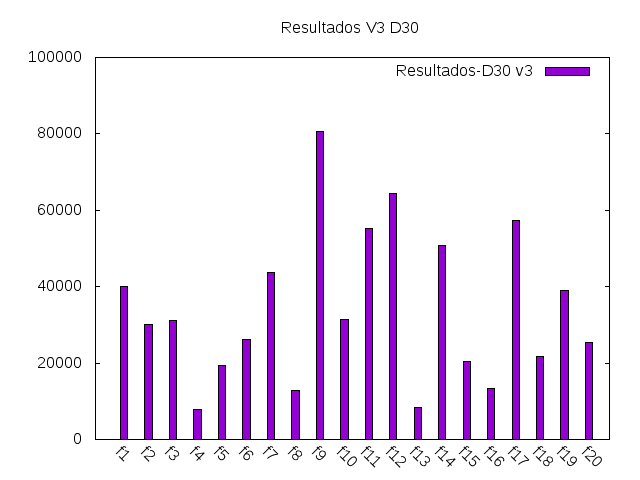
\includegraphics[scale=0.25]{./Imagenes/Resultados/resultados_v3_d30.png}
		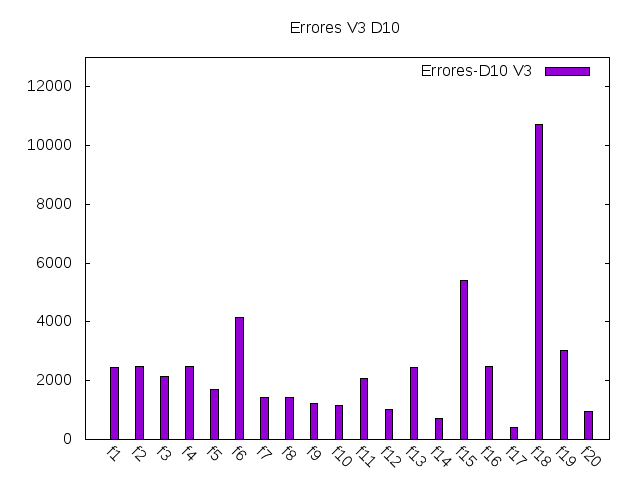
\includegraphics[scale=0.25]{./Imagenes/Errores/errores_v3_d10.png}
		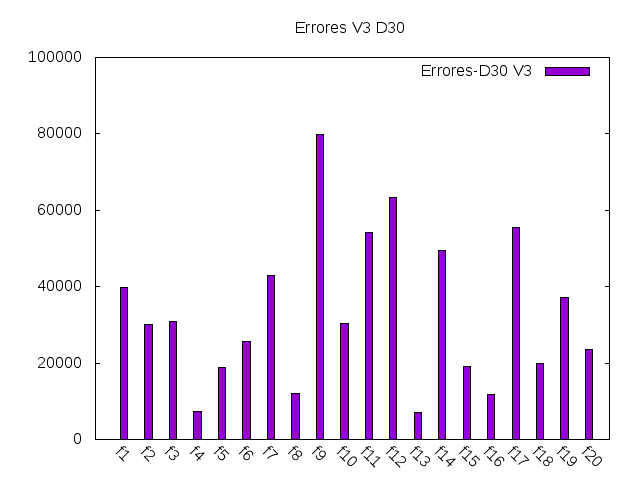
\includegraphics[scale=0.25]{./Imagenes/Errores/errores_v3_d30.png}
		
		\metroset{block=fill}
		\begin{block}{Características}
			\begin{itemize}
				\item Incorporación de la búsqueda local Solis Wets.
			\end{itemize}
		\end{block}
	\end{frame}

	\begin{frame}[fragile]{Cuarta versión}
		\centering
		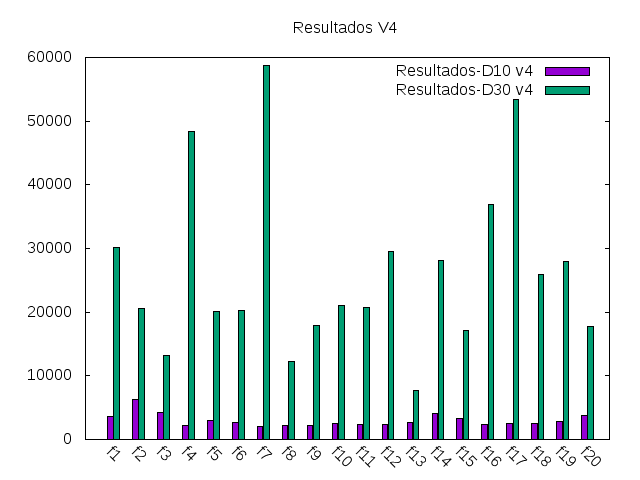
\includegraphics[scale=0.25]{./Imagenes/Resultados/resultados_v4.png}
		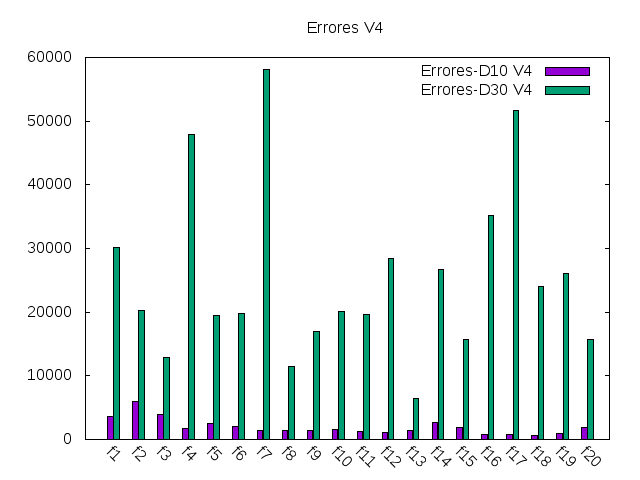
\includegraphics[scale=0.25]{./Imagenes/Errores/errores_v4.png}
		
		\metroset{block=fill}
		\begin{block}{Características}
			\begin{itemize}
				\item Incorporación de Differential Evolution.
			\end{itemize}
		\end{block}
	\end{frame}

	\begin{frame}[fragile]{Quinta versión}
		\centering
		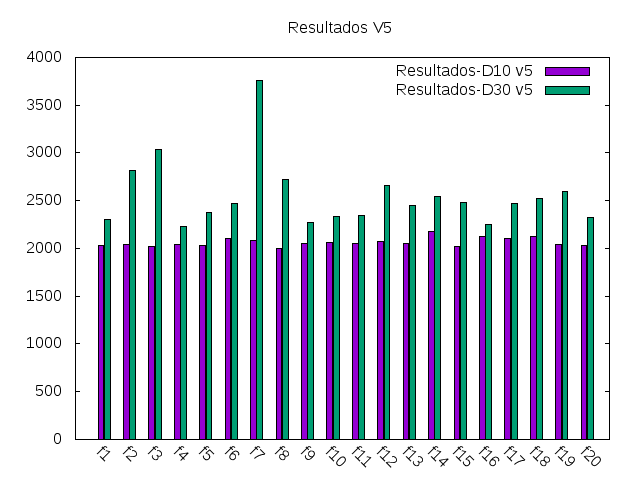
\includegraphics[scale=0.25]{./Imagenes/Resultados/resultados_v5.png}
		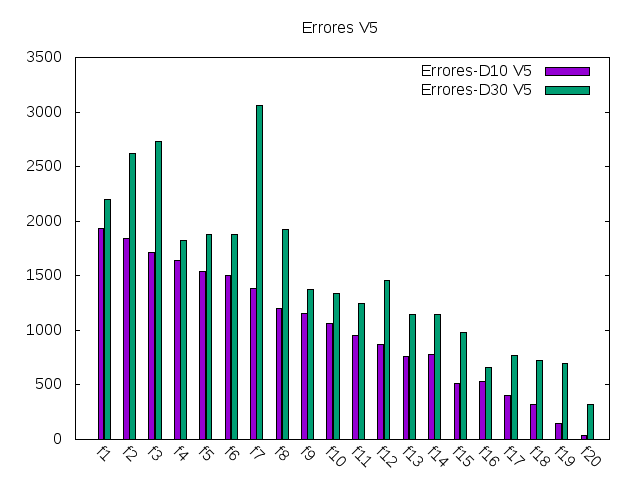
\includegraphics[scale=0.25]{./Imagenes/Errores/errores_v5.png}
		
		\metroset{block=fill}
		\begin{block}{Características}
			\begin{itemize}
				\item Sustitución de Solis Wets por CMAES.
			\end{itemize}
		\end{block}
	\end{frame}

	\begin{frame}[fragile]{Sexta versión}
		\centering
		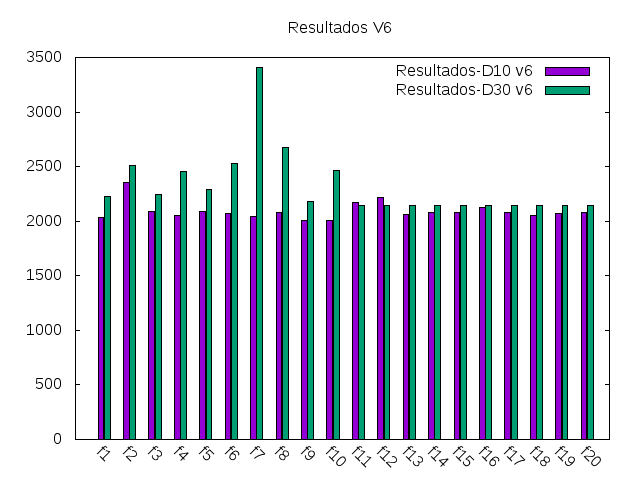
\includegraphics[scale=0.25]{./Imagenes/Resultados/resultados_v6.png}
		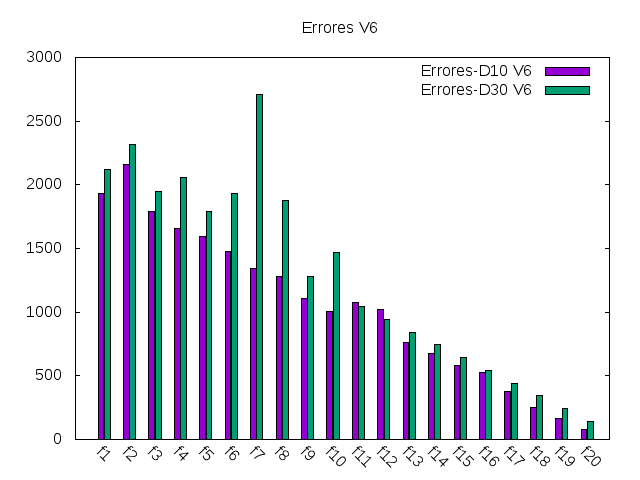
\includegraphics[scale=0.25]{./Imagenes/Errores/errores_v6.png}
		
		\metroset{block=fill}
		\begin{block}{Características}
			\begin{itemize}
				\item Aproximación a un vector aleatorio en vez de a una ballena aleatoria.
			\end{itemize}
		\end{block}
	\end{frame}

	\begin{frame}[fragile]{Progresión de las ballenas}
		\centering
		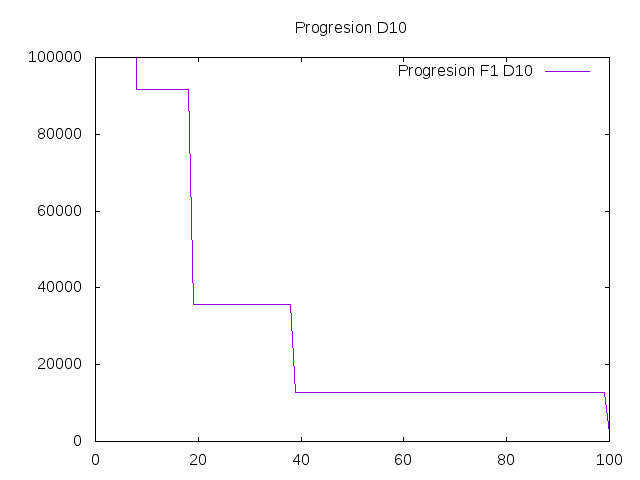
\includegraphics[scale=0.25]{./Imagenes/Progresion/progresion_mejores_10.png}
		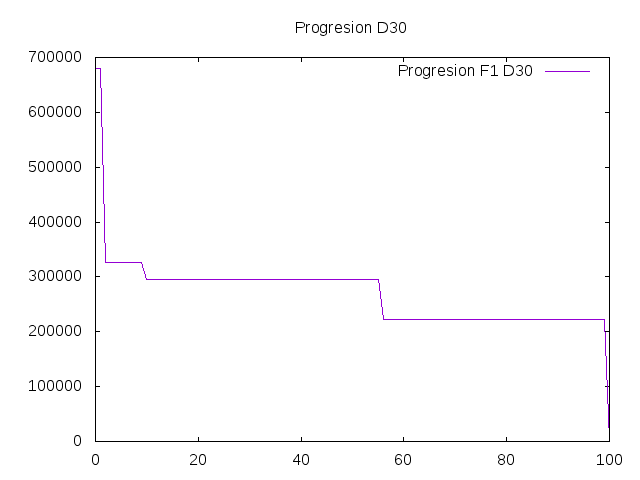
\includegraphics[scale=0.25]{./Imagenes/Progresion/progresion_mejores_30.png}
		
		\metroset{block=fill}
		\begin{block}{Comentarios}
			\begin{itemize}
				\item La mejora se produce cuando DE o CMAES se ejecutan.
				\item Aprovechamos las iteraciones del algoritmo porque mejoramos en general.
				\item Este esquema es sólo para la función 1 ya que se parecía en el resto de funciones.
			\end{itemize}
		\end{block}
	\end{frame}

	\begin{frame}[fragile]{Comparativa con los algoritmos}
		\begin{table}[!h]
			\centering
			\resizebox{200pt}{!}{
				\begin{tabular}{ | l | l | l | l | l | l | l | l | l | l | l | l | l | l | l | l | l | l | l | l | l | l | l | l  |l | l  |l | l | }
					\hline
					\underline{\textbf{Posición}} & \underline{\textbf{Clasificación D10}} & \underline{\textbf{Error}} & \underline{\textbf{Clasificación D30}} & \underline{\textbf{Error}} \\ \hline
					1 & L-SHADE & 81.2756 & iCMAES-ILS & 1440 \\ \hline
					2 & D-SHADE & 112.8402 & L-SHADE & 1470 \\ \hline
					3 & CoDE & 114.0602 & D-SHADE & 1570 \\ \hline
					4 & SHADE11 & 118.4516 & GaAPADE & 2180 \\ \hline
					5 & rmalschcma & 138.2605 & NBIPOP-aCMA-ES & 2410\\ \hline
					6 & MVMO & 140.7138 & MVMO & 2660 \\ \hline
					7 & dynNP-jDE & 165.5208 & UMOEAS & 2680 \\ \hline
					8 & JADE & 166.6920 & SHADE11 & 3050 \\ \hline
					9 & UMOEAS & 176.1225 & rmalschcma & 3180 \\ \hline
					10 & iCMAES-ILS & 185.9477 & CMLSP & 4360 \\ \hline
					11 & GaAPADE & 250.8654 & RSDE & 6070 \\ \hline
					12 & SaDE & 270.1111 & JADE & 15100 \\ \hline
					13 & NBIPOP-aCMA-ES & 281.6920 & POBL\_ADE & 23800 \\ \hline
					14 & EPSDE & 409.9321 & \textbf{WOA} & 25400 \\ \hline
					15 & RSDE & 445.5327 & CoDE & 29800 \\ \hline
					16 & DEBin & 577 & dynNP-jDE & 49500 \\ \hline
					17 & DEexp & 632 & EPSDE & 74300 \\ \hline
					18 & CMLSP & 737.2535 & OptBees & 118000 \\ \hline
					19 & OptBees & 2177.5830 & DEBin & 119000 \\ \hline
					20 & FWA-DM & 5712.6597 & FWA-DM & 286000 \\ \hline
					21 & POBL\_ADE & 19230.3251 & SaDE & 314000 \\ \hline
					22 & \textbf{WOA} & 20845.9416 & DEexp & 321000 \\ \hline
					23 & SOO+BOBYQA & 22242.966 & NRGA & 839000 \\ \hline
					24 & NRGA & 56303.5641 & SOO+BOBYQA & 2760000 \\ \hline
					25 & SOO & 11963128 & SOO & 244000000 \\ \hline
					26 & FCDE & 1719329.8 & b3e3pbest & 534000000 \\ \hline
					27 & FERDE & 144238862 & FCDE & 1800000000 \\ \hline
					28 & b3e3pbest & 227017644 & FERDE & 3640000000 \\ \hline
				\end{tabular}
			}
			\label{Ranking}
		\end{table}
	\end{frame}

	\begin{frame}[fragile]{Comparativa con el resto de algoritmos}
		\metroset{block=fill}
		\begin{block}{Comentarios}
			\begin{itemize}
				\item En dimensión 10 obtenemos malos resultados.
				\item En dimensión 30 obtenemos resultados mucho más aceptables superando a DE.
				\item El esquema de exploración con CMAES y DE añaden valor sobre el DE básico.
				\item Casi todos los algoritmos que han competido en CEC2014 están por encima.
			\end{itemize}
		\end{block}
	\end{frame}

\section{Conclusiones}

	\begin{frame}[fragile]{Conclusiones}
		\metroset{block=fill}
		\begin{block}{Conclusiones}
			\begin{itemize}
				\item Buena idea teórica pero no es eficaz en la práctica.
				\item La exploración lineal y espiral no funciona bien por sí sola.
				\item El algoritmo final ha acabado siendo un esquema CMAES-DE con reinicio de la población con una cierta probabilidad.
				\item No se encuentra en el estado del arte.
				\item Funciona mejor en dimensión 30 que en dimensión 10.
			\end{itemize}
		\end{block}
	\end{frame}

\end{document}
